\section{\hei{暑假第二周工作报告(2013.7.22-2013.7.28)}}

\subsection{\hei{上周计划}}


看dlinux的源代码,和看linux内核设计与实现。

\subsection{\hei{工作摘要}}


1)上周计划的是这周主要看dlinux的源代码,从周一到周三一直在看dlinux源代码,看了spmc\_emem.c、spmc\_thread.c和看了spmc\_pmap.c,进程和空间有着对应的关系。主要还是看了文件spmc\_pmap.c的内容,对于其中的几个函数在整体上有了初步的了解,但是对于一些判断条件(例如对pte flags位的判断)、一些函数调用不是很明白。由于工作的变动,这些问题没有继续深入的解决。


2)新的工作是关于llvm,一开始对于llvm的了解非常有限,通过这两天阅读llvm的文档,对于llvm有了初步的了解。

\begin{itemize}

\item{LLVM 是 Low Level Virtual Machine 的简称,这个库提供了与编译器相关的支持,能够进行程序语言的编译期优化、链接优化、在线编译优化、代码生成。阅读了\href{http://www.aosabook.org/en/llvm.html}{Intro to LLVM},通过对比了解了LLVM's Implementation of the Three-Phase Design(如图)。代码通过frontend的分析,检测错误后,被翻译成LLVM IR,这种IR经过一系列的分析优化,然后根据不同的机器平台,被翻译成不同的机器代码。}

\item{粗略过了一遍\href{http://llvm.org/docs/LangRef.html}{LLVM Language Reference Manual},llvm代码表示被设计成3种形式:为编译器的IR,为硬件的bitcode(字节码),还有为人类阅读的汇编表达式。LLVM变量有两种基本形式:全局变量和局部变量,全局变量以@开头,局部变量以\%开头。之后关注了Instruction Reference,了解了一些指令。例如,ret(返回指令),br(转移指令?这个还不是太明白),invoke,add(操作数是整数或向量的加法),fadd(操作数是浮点数或向量的加法)等。对于llvm指令有了大致的了解。}
\item{相比较其他的编译器,LLVM提供了5方面的能力:

1)A persistent, rich code representation:LLVM to LLVM optimizations can happen at any time.

2)native code generationtem:Generate high-quality machine code, retaining LLVM.

3)Profiling \& optimization in the field:Runtime and offline profile-driven optimizers.

4)Language independence:Low-level inst set \& types with transparent runtime.

5)Uniform whole-program optimization:Optimize across source-language boundaries.
      
}

\end{itemize}

\begin{figure}
\centering
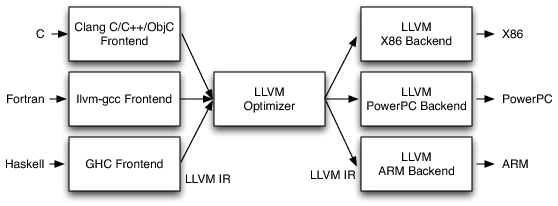
\includegraphics[width=6in]{img/LLVMCompiler1.png}
\caption{LLVMCompiler1}
\label{LLVMCompiler1}
\end{figure}

\subsection{\hei{存在的问题与不足}}


1)对于llvm的知识,还需要继续了解。


2)linux的操作还要继续熟悉。

\subsection{\hei{下一周计划}}

1)继续阅读\href{http://llvm.org/}{LLVM}文档。

2)看c++。

